\documentclass{sig-alternate-05-2015}
\usepackage{amsmath, amssymb}
% for some reason the sig document class doesn't work well with amsthm \usepackage{amsthm} 
\usepackage{thm}
\usepackage{tikz}
\usepackage[all]{xy}
\usepackage{url}

\title{A science for measuring cities: hybrid indicator frameworks for the smart city}
\author{Joshua Z. Tan, Christine Kendrick, Abhishek Dubey, Derek Loftis, and Sokwoo Rhee}
\date{\today}

\theoremstyle{plain}
\newtheorem{thm}{Theorem}[section]
\newtheorem{prop}[thm]{Proposition}
\newtheorem{cor}[thm]{Corollary}
\newtheorem{lem}[thm]{Lemma}

\theoremstyle{plain}
\newtheorem{define}{Definition}
\newtheorem{example}{Example}

\theoremstyle{remark}
\newtheorem{remark}{Remark}

% editing definitions
\newcommand{\grayout}[1]{{\color{gray}#1}}
\newcommand{\redout}[1]{{\color{red}#1}}
\newcommand{\marginnote}[1]{\marginpar{\footnotesize \color{blue}#1}}

% category theory definitions
\DeclareMathOperator{\id}{id}
\DeclareMathOperator{\dom}{dom}
\DeclareMathOperator{\cod}{cod}
\DeclareMathOperator{\dvert}{Vert}
\DeclareMathOperator{\Lax}{Lax}
\DeclareMathOperator{\Hom}{Hom}
\DeclareMathOperator{\Mor}{Mor}
\DeclareMathOperator{\Ob}{Ob}
\DeclareMathOperator{\MOb}{\lvert\mspace{2mu}\cdot\mspace{2mu}\rvert}
\DeclareMathOperator{\Tr}{Tr}
\DeclareMathOperator*{\colim}{colim\;}
\DeclareMathOperator{\Coll}{Col}

\newcommand{\Cat}[1]{\mathsf{#1}}
\def\Set{\Cat{Set}}
\def\Poset{\Cat{Poset}}
\def\DP{\Cat{DP}}
\def\DPI{\Cat{DPI}}
\def\Bool{\Cat{Bool}}
\def\Ind{\Cat{Ind}}
% end category theory definitions

% codesign definitions
\def\DP{\Cat{DP}}
\def\DPI{\Cat{DPI}}
\def\Bool{\Cat{Bool}}
\def\split{\text{split}}
\def\para{\text{par}}
\def\Conw{\text{Conw}}
\def\exec{\text{exec}}
\def\eval{\text{eval}}
\def\fix{\text{fix}}
\def\TFS{\Cat{TFS}}
\def\dom{\tn{dom}}
\def\cod{\tn{cod}}
\def\op{^{\text{op}}}
\newcommand{\funsp}{\mathsf{F}}
\newcommand{\ressp}{\mathsf{R}}
\newcommand{\impsp}{\mathsf{I}}
\newcommand{\afun}{\mathsf{f}}
\newcommand{\ares}{\mathsf{r}}
\newcommand{\adp}{\text{dp}}
% end codesign definitions

\begin{document}
\maketitle

\redout{Suggestions from Ed: make sure to motivate the math before even mentioning ``hybrid indicator frameworks'' as a solution. There are things called ``process indicators'' in systems engineering, which are a bit different from KPIs. We need a completeness theorem stating that the diagrammatic calculus for indicator frameworks actually models all possible indicator frameworks and correlations.}

\redout{Publication strategy: use this paper to focus on formalizing just indicator frameworks\emph{without mentioning the hybrid part}, with a diagrammatic calculus, and publish in the CPS week workshop. Create an application-focused paper, again without the `hybrid' part, that connects this workshop paper with the CPS Framework, and publish that in Ed's special issue. Finally, develop in late spring a full hybrid indicator framework paper.}

\begin{abstract}
An \emph{indicator} is a data source like a sensor or a census, but may also represent combinations of other indicators. For a given project or policy in a city, what are ``right'' indicators to evaluate the project's impact to the city? At the very least, the right set of indicators should be determined by comparing the trajectories of the indicators. But there are a variety of constraints that we can impose on those trajectories; the contribution of this paper is to convert knowledge about the indicators into constraints on the trajectories. We develop a mathematical theory for mapping certain classes of complex systems models, from simple `co-design' models to more complicated cyber-physical systems models, to systems of key performance indicators, and call such models \emph{hybrid indicator frameworks}. Finally, we illustrate the framework by applying it to two smart-city projects in Portland, Oregon, and Hampton Roads, Virginia.

%We first give an abstract definition of indicators as objects satisfying three properties: (1) indicators are typically generated by other indicators\footnote{can `generated' just mean take the Cartesian product of the indicator states, or do we have to capture the semantics of whatever function is used to combine the underlying indicator values?}, (2) indicators carry state as tables of data\footnote{or is the state of an indicator \emph{just} the data value at any one time?}, and (3) indicators are fundamentally things that can go ``up'' or ``down''. We then give two separate definitions of \emph{indicator frameworks} as open, discrete dynamical systems and as lax functors on monoidal categories, and show their equivalence\footnote{largely based on \url{http://128.84.21.199/pdf/1609.08086v1.pdf}}.
%
%Lastly, we develop a theory for relating a large class of complex system models, from simple `co-design' models to cyber-physical systems models to database models, to such indicator frameworks. In particular, the theory allows us to generate \emph{hybrid indicator frameworks} as structure-preserving mappings from hybrid dynamical systems to indicator frameworks.
%
%We use hybrid indicator frameworks to ground existing, ontology-based approaches to the measurement of complex systems, and apply the framework to specific examples in urban studies, including the Boston Indicators Project and the CITYKeys indicator framework for smart cities. We conclude by describing a trial implementation of the indicator framework in one or more actual cities.
\end{abstract}

\section{Introduction}
City administrators choose \emph{key performance indicators}, or KPIs, as a part of a larger effort to understand, communicate, and realize their strategic priorities. There are several strategy-setting frameworks for choosing KPIs, from balanced scorecards \cite{epstein1997balanced} to SMART \cite{doran1981there} to more specialized urban planning frameworks; in such frameworks, the KPIs are often designed in tandem with new projects, new policies, and new processes. Once chosen, they are used in program evaluation and reporting, in departmental reviews, and in request-for-proposal creation.

More recently, the advent of ``smart cities'' and the Internet of Things have given city administrations an opportunity to reform and to clarify their strategic priorities. As public services from energy grids to transportation networks to healthcare systems are automated, cities are becoming cyber-physical systems (CPS) in the true sense of the term---systems whose physical processes are profoundly integrated with computation and data. But a smart city is more than just the sum of many smart services; it the sum of many smart services and all the ways in which they interact with each other, both physically and computationally. By understanding these interactions, we can make better decisions about the services themselves, e.g. about how to optimize existing services or how to solicit new solutions. In order to understand these interactions and their data, our indicator frameworks for evaluating data must incorporate CPS models of the interactions. % we should have a story for how to abstract away processes we don't model (like social ones) ``into the data''

% [Present an example + a graphic.] Suppose we are evaluating a bus line service in New York City. In the existing KPI frameworks, the KPIs for the bus line are chosen prior to the choice of the solution, and once the KPIs are chosen, the indicator framework does not distinguish between a smart bus line and a dumb bus line (except, presumably, in the trajectory of the data from the indicators). In a hybrid indicator framework, a smart bus line generates data which links it to a larger network of related and interacting services, and is evaluated according to its effects on the entire network.

A generic indicator is a consistent source of data. Instead of beginning with individual indicators, this paper begins conceptually with \emph{indicator frameworks}: assemblages of simple indicators, however defined, which measure both physical and computational processes. The processes themselves may be modeled at various levels of abstraction. In this paper, we use a relatively simple co-design model based on work by \cite{2015arXiv151208055C}, leaving other, more general CPS models to future work. 

%\footnote{Did the process come first (in which case it should be modeled first), or did the indicators come first? In practice, cities usually come up with the indicators first. Unfortunately, sometimes indicators are chosen without understanding whether it is possible to collect the data needed for the indicator. Either assumption is valid. They define different queries one can run against a hybrid indicator framework.}
 
% Traditional complex systems theory focuses on the idea of interconnection, or ``internal composition'': complicated structures are modeled according to the ordering or graphing of their internal modules. A core idea of this paper is composition in the sense of ``external composition'': in situations where many, heterogeneous models are used to describe a larger model, as in models of cities and other cyber-physical systems, we must also to develop the interconnections between these different models. % Doing so can lead to [more comprehensive and more elastic tools for planning and modeling.]

% [Add discussion of the practical benefits. In particular, discuss how it improves one of these scenarios: (1) Plug in a cyber-physical system (or a codesign diagram), turn the crank, and get a list of indicators? (2) Plug in a list of indicators and get out a `better' list of indicators? (3) Plug in a solution and get out a list of indicators?] 

Our work is driven by practical considerations in project governance at the Global City Teams Challenge \cite{7515058}, a U.S. federal government smart city program led by the National Institute of Standards and Technology (NIST) with participation from over 120 cities and 300 organizations worldwide. By linking indicator frameworks with complex system models, we hope to better account for second-order effects of policies and projects, allowing policymakers to use multiple levers in project management. We also allow easier knowledge retention and make it easier to consume complicated, inaccessible models that typically exist in academia or with solution providers. \redout{For example, consider a city that is deploying two projects: one which improves transit signal priority so that travel times for people are reduced and another which increases and improves crosswalks with smart lighting to reduce traffic-related fatalities. If people feel safer, there could be a positive net gain in individuals who will also ride transit and travel times could be reduced further showing a co-benefit or positive trajectory on both indicators. However, depending on the actual design of the roadway corridor, increased pedestrian crossings could impede traffic as transit always has to stop and travel times may stay neutral or even increase, showing an unexpected negative effect on a separate indicator. Co-benefits across indicators can be useful in helping invest in the right projects. Conversely, if two projects have opposite effects on two indicators, then a city can understand why they did not see the effect the planned project was projected to have. If such interactions can be identified beforehand, then an improved set of indicators can be developed and/or the project design can be adjusted.} 

% [Put in if we have time.] \emph{What we are not doing}: we are not doing some sort of automated reasoning. We are trying to take processes that are already underway, and formalize them so that the processes are easier to scale and to integrate.

\section{Background}
Modern cities are composed of several highly networked cyber-physical systems from the electric grid to the water supply to transportation Networks. These are integrated together to provide services essential for city residents. Individually, each service or city process can be thought of as a coupled feedback system where a software subsystem controls a physical subsystem by collecting data on it through sensors and providing the necessary control action. For example, the heating system of a building measures the temperature of the building via sensors and then controls the heater state.  The output from the software subsystem is assumed to pass through the actuation subsystem, which converts the software output into control actions (mechanical inputs)  and then imposes them onto the physical subsystem. The control action changes with the state of physical subsystem. Consequently, the state of the physical subsystem changes with time due to the control action from the software subsystem. Thus, each CPS in essence is a hybrid system with both discrete and continuous dynamics. 

% Each connection between software and physical subsystems is an indicator.

Compared to other cyber-physical systems such as robotics, manufacturing, and even aviation, cities are more complex, more diverse, and more unpredictable. This is due to the fact that cities are a composition of these multi-domain CPS, wherein the interaction between each of the domain is not strictly engineered as in the subcomponents of a robotic system or an aircraft. In a traditional engineering domain like robotics, the CPS can be analyzed using dynamical systems theory, with the assumption that the systems are typically in equilibrium and they can be controlled with the typical tools of planning and management. However, in a city system, which is influenced by social physics and where the interactions are orchestrated via humans, the traditional models are often found lacking \cite{batty2012smart,batty2012building}. This is primarily due to the unpredictable nature of humans, whose behavior ranges from irrational and unpredictable at best, to intelligent, deceptive, and malicious at worst \cite{munir2013cyber,10.1109/MC.2013.149}. Cities are notoriously hard to model and comprehend with closed form analytical methods. The sheer scale, range of actions and diversity adds another level of complexity.

For example, the Architecture Analysis and Design Language (AADL)~\cite{AADL_Intro:06,Feiler_AADL:06} is a standard developed by the Society of Automotive Engineers. Originally developed for aerospace systems, the standard is applicable to the model-based specification and analysis of embedded real-time systems and systems of systems. It has comprehensive support for modeling a variety of component types and their interactions. Component abstractions in AADL consist of software components, computational hardware, and the overall system. Different interaction patterns between components are supported in AADL.  Using AADL it is possible to conduct analysis for a variety of critical system properties, such as performance, schedulability and reliability. Other general-purpose approaches similar to AADL are OMG's SysML and OMG's MARTE profile for UML.   SysML~\cite{hause2006sysml} is a general-purpose modeling language for systems engineering. SysML leverages a subset of the Unified Modeling Language (UML) while extending it with capabilities needed to model complex systems engineering problems, which is called the SysML profile for UML. The extensions enable engineering analysis.  The Modeling and Analysis of Real-time and Embedded (MARTE) systems~\cite{MARTE_v1.1:11} is a UML profile to extend UML to support the model-driven development of real-time and embedded systems. However, it is difficult to use these modeling and description languages for cities because of uncertainty in subsystem interactions. 

Without such integrated models it is difficult to understand the integrated performance impact of  various decisions taken at the level of different city systems. Therefore, traditionally city based systems have been studied using simulations, game-theoretic models and agent-based models. Game-theoretic models \cite{7028565,Rosenschein:1994:RED:180311} describe the problem by modeling the individual agents and describing their interactions as negotiations, and then using several mechanisms to arrive at a globally optimal solution. Initially, game theoretic methods assumed that all agents worked together collaboratively, but they have also been formulated to use an adversarial model, especially in economics, business, and market strategy. Another approach to studying and modeling these types of problems is agent-based modeling and simulation \cite{karnouskos2009simulation,batty2012smart}, which uses individual, communicating agents to evaluate system properties. This is the approach used in the MATSim (``Multi-Agent Transport Simulation Toolkit'') toolkit \cite{balmer2008agent,matsim}. This toolkit implements a multi-agent transport simulator that can be used to describe the activities of agents, which in turn provides a demand model. Combined with a set of origination/destination maps and capacity plans, the toolkit can simulate the system performance.

Another alternative is to use a data-driven, human-in-the-loop approach to analyzing cities. For example, \cite{7501714} describes how the data collected from various public transportation vehicles can be used to analyze the performance of transit systems. The authors describe a data-driven performance measurement tool for waste management in \cite{zaman2013zero}. \cite{williams2014measuring} describes various performance indicators for low carbon cities in china. The data-driven approach is also useful for better understanding system anomalies and behaviors \cite{qin2012survey,chandola2009anomaly}. System experts and engineers can use the information gleaned from this data to update operations procedures and even redesign some of the city systems. Data-driven approaches have now been adopted almost universally across major cities in the world, and have influenced the creation of many indicator frameworks, from CITYKeys \cite{citykeys} in the European Union to ISO/TS 37151 \cite{iso} by the International Standards Organization. Such indicator frameworks, however, are essentially ad hoc: they give a light-weight classification of indicators along hierarchies, and focus much more on justifying the inclusion of individual indicators into a framework than their large-scale interrelation.

We subscribe to a data-driven approach insofar as we begin with a technical definition of indicator framework. Concretely, however, it is the \emph{lack} of sufficient data that has driven our inclusion of CPS and other tools from dynamical systems theory into indicator frameworks. The processes of a city are simply too complex to measure directly. If we had the data, we would just generate a correlation matrix with it. Unfortunately, we do not, so we must develop models to make up for that deficit.

% The data-driven approach has also led to the use of indicator frameworks .... [Josh connect this]

\section{Hybrid Indicator Frameworks}
\emph{Indicators} convey information in a consistent way across time and across different systems. They may be sensors, scientific measurements, or arbitrary database columns, so long as they can ``indicate''---i.e., go up or down. Indicators may be also associated to processes; to say that an indicator is a ``key performance'' indicator is just to state that the indicator is associated to some given process or processes. For the purposes of this paper, we will represent indicators as objects in a given sort of \emph{category}, and trajectories as finite sequences valued in partially-ordered sets. % Philosophically, the ``use�� of data is that it represents some underlying process or project, and to say that data comes from an indicator is to say, at a minimum, that the data comes from a consistent source or apparatus, e.g. a scientific experiment.

\subsection{Preliminaries}
First, some definitions.

A \emph{category} $\mathcal{C}$ is defined by the following data:
\begin{enumerate}
\item A collection of objects, called the objects of $\mathcal{C}$.
\item A collection of maps between any two objects $c,c' \in \Ob \mathcal{C}$, called the arrows from $c$ to $c'$, e.g. $f : c \to c'$.
\item A composition rule between arrows, written $g \circ f$ for first $f$ then $g$, satisfying an identity axiom and an associativity axiom.
\end{enumerate}
% The collection of all categories itself forms a category, and in this category the arrows are called \emph{functors}. Importantly, functors must say not only what happens to the objects of a category, but also what happens to its arrows. 
A \emph{functor} from a category $\mathcal{C}$ to a category $\mathcal{D}$ is a mapping $F : \mathcal{C} \to \mathcal{D}$ that associates each object in $\mathcal{C}$ to an object in $\mathcal{D}$, and associates each arrow $f: c \to c'$ to an arrow $F(f) : F(c) \to F(c')$ in such a way that respects the composition rule.

Category theory is a branch of mathematics originally used to translate results from one area of mathematics to another, e.g. from topology to algebra. It has now been applied to subjects ranging from quantum mechanics \cite{2008arXiv0808.1023A, 2009arXiv0903.0340B} to dynamical systems modeling \cite{2015arXiv150207380S, 2016arXiv160905382F} to database theory \cite{2010arXiv1009.1166S} to general models of processes \cite{2015arXiv150405625B} and, most recently, to cyber-physical systems \cite{2016arXiv160908086S}. For an exposition of category theory, we recommend the reader to any of the introductory texts for computer scientists \cite{awodey}, engineers \cite{spivak}, or for mathematicians \cite{maclane}.

A \emph{partially-ordered set}, or poset, is a set with a relation $\leq$ satisfying reflexivity, anti-symmetry, and transitivity. A monotone map between posets is an order-preserving function, i.e. $f$ is monotone iff $a \leq b \Rightarrow f(a) \leq f(b)$. An antitone function is an order-reversing function, i.e. $a \leq b \Rightarrow f(a) \geq f(b)$.

A \emph{(co)-design problem} is a certain kind of optimization problem involving \emph{functionalities} $\funsp$ and \emph{resources} $\ressp$, with the constraint that $\funsp$ and $\ressp$ are posets. Each design problem, $\adp$, represents an optimization problem for a particular process whose inputs are resources in $\ressp$ and whose outputs are functionalities in $\funsp$. Importantly, primitive design problems can be composed to create larger (co-)design problems by series, parallel, and loop operations.

The expression $[\adp](\afun, \ares)$ may be thought of as a statement of the form, ``given functionality $\afun$ and $\ares$, is there an implementation that delivers $\afun$ at cost $\ares$?'' We refer to \cite{censi} for the details. In this paper, we will mainly use the fact that design problems form a category, $\DP$, whose objects are posets and arrows are profunctors \[[\adp] : \funsp\op \times \ressp \to \Bool.\] In particular, we will be analyzing co-design diagrams in the form of Figure~\ref{fig:codesign1}.

\begin{figure}[h]\label{fig:codesign1}
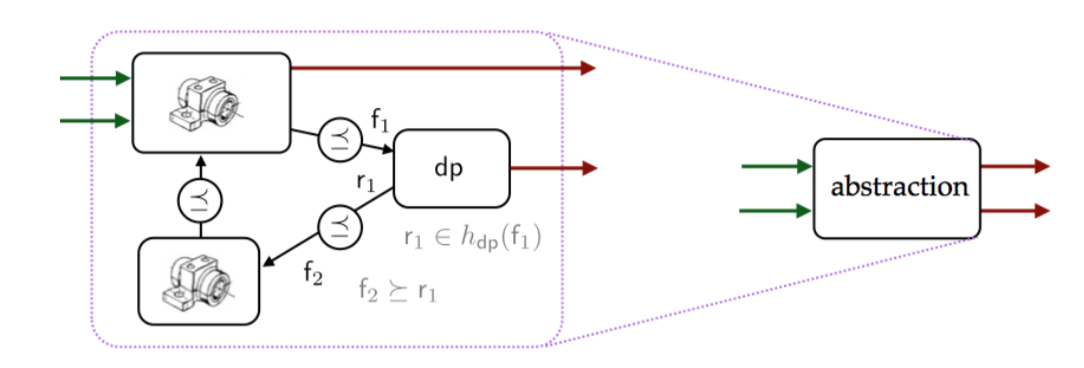
\includegraphics[width=\linewidth]{mcdp_1}
\caption{Multiple design problems compose to form one co-design problem.}
\end{figure}

\subsection{Indicator Frameworks}
\begin{define}An \emph{indicator framework} is a small category $\mathcal{C}$ with the following conventions:
\begin{enumerate}
\item An object $c$ in $\mathcal{C}$ is a Boolean set $\{\uparrow, \downarrow\}$ called an \emph{indicator} in $\mathcal{C}$.
\item Each arrow of $\mathcal{C}$ is a function $f: c \to c'$ called a \emph{(simple) correlation} from $c$ to $c'$. % We can eventually broaden this!
\item The identity map $\id_c : c \to c$ is called the \emph{primary id} on $c$. On most indicators, the primary id is time.
\item An object $c$ in $\mathcal{C}$ with no outgoing arrows is called an \emph{indicator type}.
\end{enumerate}
A \emph{trajectory} on $\mathcal{C}$ is a functor $T : \mathcal{C} \to \Poset_W$, where $\Poset_W$ is the category of posets and monotone maps between posets satisfying a ``windowing'' condition: indicator values can be mapped to other indicator values only if their time values are within some $\epsilon$-window of each other. 

For any indicator $c \in \mathcal{C}$, an element $x \in T(c)$ is called an \emph{indicator value}. 
\end{define}

There is an analogy between the above and the definition of a database schema in \cite{2010arXiv1009.1166S}; this is to be expected since most indicator frameworks are, essentially, views into a database. The difference is that we are not tracking parent-child relations in the sense of the foreign keys of a database, but linear relations in the sense of indicators going `up' and `down'.

Indicator frameworks can be graphed as categories, while trajectories can be written down as collections of tables. As shorthand, we use green arrows to represent positive correlations $\uparrow \; \mapsto \; \uparrow$, and red arrows to represent negative correlations $\uparrow \; \mapsto \; \downarrow$, as in the following example:
\[
\xymatrix{
        \text{Traffic Volume} \ar@[green][d] \ar@[green][rd] & \text{Wind Speed} \ar@[red][d] \\
        \text{Mobile Sources} \ar@[green][r]  & \text{NO$_2$ Levels}
        }
\]
\begin{center}
\begin{tabular}{| c | c |}
  \hline
  \multicolumn{2}{|c|}{\textbf{Traffic Volume}} \\ \hline
  \textbf{Time} & \textbf{Indicator Value} \\ \hline
  09:00:00 10-13-2016 & High \\ \hline
  10:00:00 10-13-2016 & Medium \\ \hline
  11:00:00 10-13-2016 & Low  \\ \hline
  \hline
  \multicolumn{2}{|c|}{\textbf{NO$_2$ Levels}} \\ \hline
  \textbf{Time} & \textbf{Indicator Value} \\ \hline
  09:00:00 10-13-2016 & 11 ppb \\ \hline
  10:00:00 10-13-2016 & 10 ppb \\ \hline
  11:00:00 10-13-2016 & 7 ppb \\ \hline
\end{tabular}
\end{center}
%Note: to make sure that $T(c)$ is always a poset, we have to consider time separately (this makes sense, if one recalls that it is, essentially, a primary key). 
 
Each correlation is, in effect, a constraint on the possible trajectories of the indicators. To see this, recall that a trajectory must satisfy the formal definition of a functor. In the example, this amounts to showing that the diagram below (and others like it) commutes: $T \circ f = T(f) \circ T$.
\[
\xymatrix{
        \text{Traffic Volume} \ar@[green][r]^f \ar@{|->}[d]_T & \text{NO$_2$ Levels} \ar@{|->}[d]^T \\
        (H, M, L) \ar[r]_{T(f)} & (11,10,7)
        }
\]
Fix some $\epsilon > 0$. In the case above, the only monotone map satisfying the windowing condition is $(H \mapsto 11, M \mapsto 10, L \mapsto 7)$. It exists, so the constraint is satisfied. Similarly, if $f$ had been a negative correlation, we would have had to find an antitone map satisfying the windowing condition. Note that as we increase the $\epsilon$-window, we always increase the number of possible monotone and antitone maps. This is important in case our data values do not match very nicely in time, but if we take it too far, our $\epsilon$-windowed correlations become useless.

Vice versa, given a set of times and indicator values---i.e. a mapping $T : \Ob \mathcal{C} \to \Poset_W$---we can also check whether those indicator values satisfy the constraints implied by the presence of the arrows in the indicator framework.

% We want to model hierarchical indicator frameworks, and separately we want to make it monoidal (so we can achieve nice mappings from the monoidal category DP). Can we do both by defining nested indicator frameworks?

\begin{define}A \emph{hybrid indicator framework} is a functor from any category to an indicator framework $\mathcal{C}$.\end{define}

The key point here is that \emph{any} model which can be formulated as a category can be used to power a hybrid indicator framework. In the rest of this section, we will build an example using the category of design problems, $\DP$, as our modeling category.

Recall our motivating question: what is the right set of indicators to evaluate \emph{a given solution}? We have chosen design problems as our modeling category in particular because a design naturally posits the possible trajectories of a given complex system---a natural dynamical system concept---as possible \emph{solutions} to that system. Hybrid indicator frameworks may be thought of as answering the opposite question: given a possible solution as input, or rather a whole space of possible solutions in the form of a co-design diagram, what are the possible trajectories of our indicators, given how we expect them to be correlated?

\begin{figure}[h]\label{fig:codesign2}
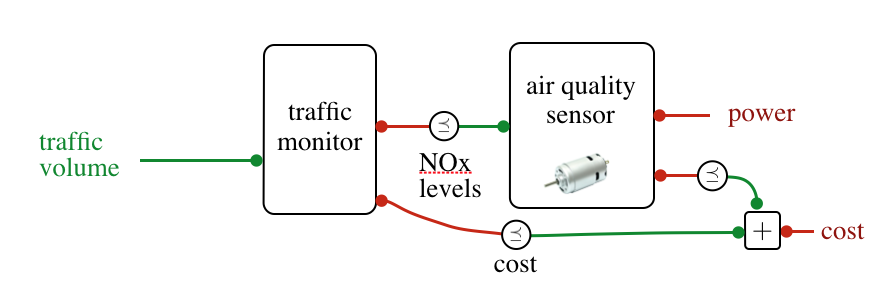
\includegraphics[width=\linewidth]{sensor}
\caption{A simple co-design diagram for a sensor and traffic monitor.}
\end{figure}

As mentioned before, design problems form a category, $\DP$, whose objects are posets (interpreted as resources) and arrows are design problems. Suppose that one of the functionalities provided by a traffic sensor is a pedestrian count, which is then consumed by a traffic computer. The sensor and the traffic computer are processes, and the indicator value of that sensor is a functionality provided by the sensor, and a resource consumed by the traffic computer. Formally, a co-design diagram thinks of each process---what goes inside the box---as a profunctor to $\Bool$ (essentially, this is a $\Bool$-valued square matrix with columns all the possible values of the sensor), but we will not really use this fact. 

In other words, the productive use of constructing a co-design diagram is that it forces us to consider the interaction between processes.

Intuitively, the relationship between a co-design diagram $\mathcal{D}$ and an indicator framework $\mathcal{C}$ is simple: each wire in the diagram corresponds to an indicator in $\mathcal{C}$, and each box attached to the wire corresponds to some process associated with that indicator. More formally, for any given trajectory $T$ on $\mathcal{C}$, a functor $H$ from $\DP$ to $\mathcal{C}$ is defined by
\begin{align*}
P \in \Ob \DP \quad &\longmapsto\quad c \in \Ob \mathcal{C} \text{ such that } T(c) = P \\
\adp : P \to P' \quad&\longmapsto\quad f : P \to P'
\end{align*}
One can check that this definition respects the composition in $\adp$. If we interpret correlations in $\mathcal{C}$ as constraints on the possible trajectories of indicator values, then literally the mapping above is lifting design problems---which are used to model interactions (in this case, simple input-output interactions) between processes---to constraints on the trajectories. % What about the other structures, e.g. the monoidal product or the trace?!?!

% The indicator category, $\Ind$, is defined by the following: morphisms are profunctors to $\Bool$---essentially, each morphism captures whether an increase in one indicator does or does not correspond to an increase in another indicator. $\Ind$ can be thought of as a generalization of the standard correlation matrix whose rows and columns are the indicators and whose entries are the correlations between the indicators� data values. It is a generalization since the state sets are not necessarily vector spaces, nor are the relationships necessarily linear.

\section{Applications}
Hybrid indicator frameworks are general enough to support many existing indicator frameworks for cities, including examples such as CITYKeys \cite{citykeys} or ISO/TS 37151 \cite{iso} where the key contextual structure is simply hierarchical grouping; one only needs to write down a category that captures the hierarchical structure, e.g. an operad.

The remainder of this section is dedicated to exploring two ongoing implementations of the framework: Portland, Oregon and Hampton Roads, Virginia.

\begin{figure*}[h!]
  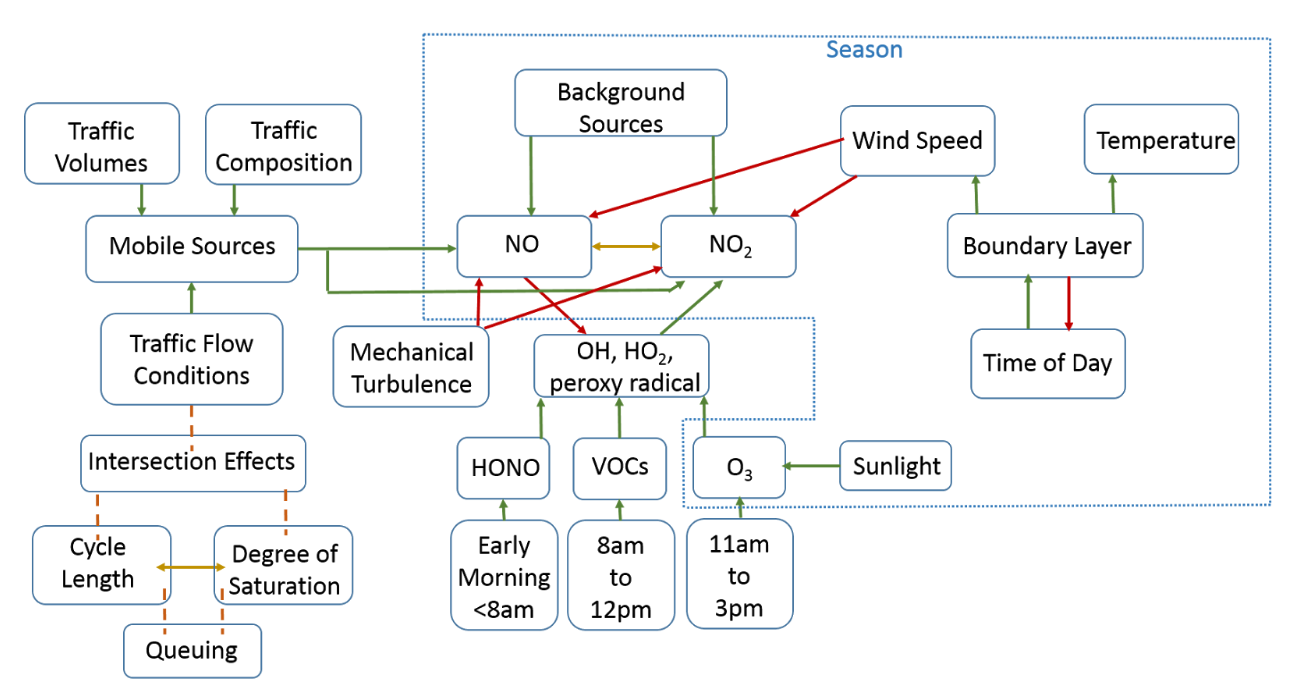
\includegraphics[width=\textwidth]{portland}
  \caption{Roadside NOx conceptual model with hypothesized relationships to variables that may alter roadside NOx concentrations. Green represents a positive correlation, red represents a negative correlation, orange represents inconclusive.}
  \label{fig:portland}
\end{figure*}

\subsection{Portland, Oregon}
The City of Portland (specifically, the Bureau of Planning and Sustainability and the Bureau of Transportation) is investigating how networks of low-cost air quality sensors can be used to improve real-time understanding of transportation-related pollution along roadway corridors. Using such data, Portland would like to evaluate the impacts on air quality and climate-related variables from transportation solutions such as improved transit signal priority, improved traffic signal coordination, increased electrification of the urban fleet, and truck priority signaling. 

Reductions in traffic-related pollution and greenhouse gas emissions are not the only indicators Portland needs to evaluate. Portland's transportation policies are also aiming to reduce traffic-related fatalities, travel delay for people and freight, and understand how changes in the transportation system affect gross regional product. These indicators of interest are components of multiple systems/models present in the urban environment including urban air quality, transportation network, human activity patterns, freight network and the economy. A final outcome/next step of this paper's work will be to determine (a) how the Portland performance indicators are impacted directly by the various transportation projects (positively, negatively, or no effect) and (b) how the indicators are impacted by effects that are a result of a change in another indicator, thus defining how the indicators are related to each other. 

In order to move towards this overlay of multiple models and identify the interactions between indicators across several urban systems, first a diagram of the urban air quality system focusing on roadside nitrogen oxides (NOx) concentrations was compiled based on knowledge from the subject matter expert, an air quality scientist, shown in Figure~\ref{fig:portland}. This diagram serves several purposes; identify all of the possible variables or processes that can change the concentrations of roadside NOx, identify which variables can or cannot be measured, and which variables have existing data sources that can be leveraged. 

In Figure~\ref{fig:portland}, NO, NO$_2$, O$_3$, wind speed, sunlight, and temperature are all variables that can be assessed with roadside sensor and background instrument measurements. Other variables like HONO and VOCs are not species that are measured at the roadside or even at background monitoring stations regularly but time of day could be used as a proxy to understand certain trends in NO and NO$_2$. Background monitoring stations can be used to assess background concentrations of NO and NO$_2$ which will not provide an estimate of emissions as a result of specific background sources but can still provide some information on regional levels of pollution separate from the localized roadway's mobile source contribution. 

So far, we have only described an indicator framework, not a hybrid indicator framework. The next step is to integrate the diagram above with a co-design diagram. This consists in defining relationships between (a) Portland's transportation solutions and indicators and (b) between the indicators themselves, i.e. to produce a similar diagram as Figure~\ref{fig:portland} but focused in on the traffic volume, composition, and traffic signal system side and other components of the transportation system compiled by a transportation subject matter expert. 

%Traffic volumes are commonly available for roadways, but depending on the traffic signal control system in place and protocols for the city, the volume data from loop detectors is not always stored or logged. Measurements of traffic signal operation such as cycle length, occupancy, degree of saturation will also be dependent on the traffic signal control system in place. Traffic composition is rarely measured continuously unless inductor loops are set-up in pairs and the City is logging the length of vehicles passing across the pair of loop detectors. Another method by which traffic composition data can be achieved is if the City is using some type of camera or radar device for detection at a mid-block location which can measure the length of vehicles passing by. Such measurements often require calibration, validation, and fine-tuning to set the best bin lengths to categorize traffic composition accurately. 
%
%Scientists, researchers, and regulators are the ones looking at concentrations of the various air pollutants and the meteorological variables depicted in Figure~\ref{fig:portland}. City transportation engineers are looking at the traffic volumes and traffic signal operations data. As mentioned some of the traffic signal operations and traffic composition data are only assessed during a study, implementation of a new detection technique, and/or when designing a new timing plan and are not necessarily variables that are assessed on a regular basis. City and regional planners use estimates of traffic volume data and traffic composition data for long-term strategic and urban planning policies but not at the scale of a roadway by roadway estimate. 

\begin{figure*}[h!]
  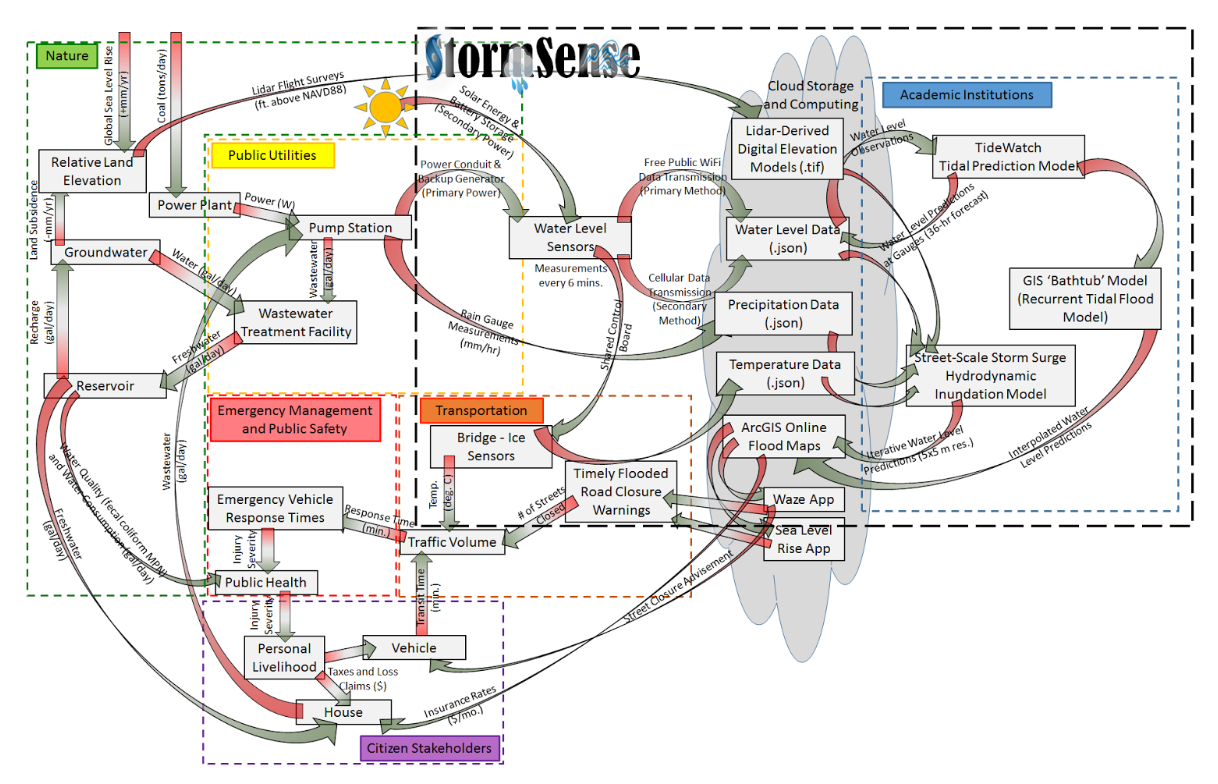
\includegraphics[width=\textwidth]{stormsense}
  \caption{Theoretical co-design diagram depicting a flood prediction methodology with hypothetically-related variables in a generalized smart city. Color coded regions represent interrelated elements of inundation prediction and disaster management. Red sections of arrows represent outputs, while green arrows represent inputs; direction of arrows suggest general flow gradient of information or resources.}
  \label{fig:stormsense}
\end{figure*}

\subsection{Hampton Roads, Virginia}
The following example is derived from the StormSense group, composed of the Virginia Institute of Marine Science (VIMS) at the College of William and Mary and many of the cities in the Greater Hampton Roads Region of Tidewater Virginia, including: Newport News, Virginia Beach, Norfolk, Hampton, Chesapeake, Portsmouth, Williamsburg, and York County. 

Hampton Roads, Virginia, is deploying a network of IoT-enabled water-level sensors, called StormSense, in order to enhance its emergency preparedness for extreme and recurrent flooding. Developed by VIMS, StormSense is a complex system that integrates these indicators with urban-scale hydrodynamic flood modeling and forecasting in the Chesapeake Bay. These models are then used to enhance emergency preparedness for flooding resulting from storm surge, rain, and tides.
 
% Hampton Roads, VA is an area regularly impacted by recurrent tidal flooding with a burgeoning population of >1.7 million people, living and traveling on roads exposed to severe and increasing frequent chronic �nuisance� flooding (Ezer and Atkinson, 2014). The region includes more than 400,000 properties exposed to flood or storm surge inundation, making it the second-largest population center in the U.S. at risk from sea level rise (CoreLogic, 2015; Boon, Brubaker and Forrest, 2010) after New Orleans, LA. Upon calibration of the initial suite of sensors throughout Hampton Roads, StormSense endeavors to develop urban-scale hydrodynamic models embedded with lidar-derived topography and building footprints within the computational grid mesh framework with the interest of developing an operational forecast model to enhance the capability of communities to prepare and respond to the disastrous impacts of sea level rise and coastal flooding in ways that are replicable, scalable, measurable, and can make a comparable difference worldwide.
 
The StormSense instance of the hybrid indicator framework centers around a generic smart city functioning as a networked cyber-physical system informed by flood predictions from a hydrodynamic model up to 36 hours prior to an inundation event. In this framework, depicted in Figure~\ref{fig:stormsense}, all components and their constituent variables (represented alongside arrows with units; as appropriate) associate with each other and are locally and globally networked in the co-design diagram. The essential elements of the StormSense flood modeling hybrid indicator framework relate to many divisions of the modern-day smart city, their constituent citizen stakeholders, natural systems and the academic research at the cross-section of these systems (color coded regions of Figure~\ref{fig:stormsense}).

\section{Discussion}
In this paper, we have developed a simple, categorical approach for combining indicator frameworks and complex system models. We have done so with the goal of predicting and measuring the impacts of a smart-city solution to a city, including possible unintended consequences. The framework was designed to provide technology providers and end-users, including local governments, a way to identify the relevant key performance indicators and to assess in advance the changes to the indicators after the deployment of solution. By using complex system models of city processes and their interactions, we can identify relevant indicators even as systems scale up in complexity. Two examples from real-world smart-city projects were introduced to demonstrate the applicability of the method, and they showed how the process of identifying relationships between indicators can be decomposed through the creation of a diagram and then the mapping of that diagram to an indicator framework.

At this point, the relationships of indicators are described only at the conceptual level, and correlations were defined with only a simplified ``up-down'' semantics. Obviously, the relationships between indicators could be nonlinear, and additional analysis and research will be necessary to suggest a more concrete method for formulating such relationships. In the case that the relationships are nonlinear or explicit solutions cannot be found, simulation-based methods may be used to track and assess the movements of the KPIs. We expect that the system modeling and decomposition approach used here will need to be further refined and reformulated.

Concretely, we expect to implement and verify hybrid indicator frameworks over the next year in a subset of the 100+ projects in NIST's Global City Teams Challenge. The proposed indicator framework will be used to assess the impacts of the solutions to the city and communities, and the validity of the framework will be verified by comparing its predictions against the actual data collects after each projects' completion.

\section{Acknowledgements}
We would like to thank David Spivak and Andrea Censi for conversations on category theory, as well as Bilin and Levent Guvenc for their contributions to the examples.

\bibliographystyle{abbrv}
\bibliography{paper} 

\end{document},